\documentclass[a4paper]{book}
\usepackage{makeidx}
\usepackage{graphicx}
\usepackage{multicol}
\usepackage{float}
\usepackage{listings}
\usepackage{color}
\usepackage{ifthen}
\usepackage[table]{xcolor}
\usepackage{textcomp}
\usepackage{alltt}
\usepackage{ifpdf}
\ifpdf
\usepackage[pdftex,
            pagebackref=true,
            colorlinks=true,
            linkcolor=blue,
            unicode
           ]{hyperref}
\else
\usepackage[ps2pdf,
            pagebackref=true,
            colorlinks=true,
            linkcolor=blue,
            unicode
           ]{hyperref}
\usepackage{pspicture}
\fi
\usepackage[utf8]{inputenc}
\usepackage[spanish]{babel}
\usepackage{mathptmx}
\usepackage[scaled=.90]{helvet}
\usepackage{courier}
\usepackage{sectsty}
\usepackage[titles]{tocloft}
\usepackage{doxygen}
\lstset{language=C++,inputencoding=utf8,basicstyle=\footnotesize,breaklines=true,breakatwhitespace=true,tabsize=8,numbers=left }
\makeindex
\setcounter{tocdepth}{3}
\renewcommand{\footrulewidth}{0.4pt}
\renewcommand{\familydefault}{\sfdefault}
\begin{document}
\hypersetup{pageanchor=false}
\begin{titlepage}
\vspace*{7cm}
\begin{center}
{\Large Filtro FIR en C \\[1ex]\large 1.0 }\\
\vspace*{1cm}
{\large Generado por Doxygen 1.7.4}\\
\vspace*{0.5cm}
{\small Miércoles, 2 de Noviembre de 2011 11:59:29}\\
\end{center}
\end{titlepage}
\clearemptydoublepage
\pagenumbering{roman}
\tableofcontents
\clearemptydoublepage
\pagenumbering{arabic}
\hypersetup{pageanchor=true}
\chapter{Indice de archivos}
\section{Lista de archivos}
Lista de todos los archivos documentados y con descripciones breves:\begin{DoxyCompactList}
\item\contentsline{section}{\hyperlink{fir_8c}{fir.c} (Implementa las funciones de inicialzación del filtro y la función de filtrado )}{\pageref{fir_8c}}{}
\item\contentsline{section}{\hyperlink{fir_8h}{fir.h} (Implementa las funciones de inicialzación del filtro y la función de filtrado )}{\pageref{fir_8h}}{}
\item\contentsline{section}{\hyperlink{genera__senales_8c}{genera\_\-senales.c} (Genera señales sintéticas para la prueba de la implementación del filtro FIR. Genera señales tipo escalón e impulso )}{\pageref{genera__senales_8c}}{}
\item\contentsline{section}{\hyperlink{genera__senales_8h}{genera\_\-senales.h} (Genera señales sintéticas para la prueba de la implementación del filtro FIR. Genera señales tipo escalón e impulso )}{\pageref{genera__senales_8h}}{}
\item\contentsline{section}{\hyperlink{testfir_8c}{testfir.c} (Programa para probar el filtro FIR implementado )}{\pageref{testfir_8c}}{}
\end{DoxyCompactList}

\chapter{Documentación de archivos}
\hypertarget{fir_8c}{
\section{Referencia del Archivo fir.c}
\label{fir_8c}\index{fir.c@{fir.c}}
}


Implementa las funciones de inicialzación del filtro y la función de filtrado.  


{\ttfamily \#include \char`\"{}fir.h\char`\"{}}\par
Dependencia gráfica adjunta para fir.c:\nopagebreak
\begin{figure}[H]
\begin{center}
\leavevmode
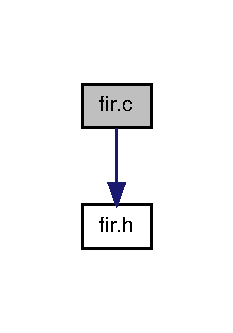
\includegraphics[width=112pt]{fir_8c__incl}
\end{center}
\end{figure}
\subsection*{Funciones}
\begin{DoxyCompactItemize}
\item 
void \hyperlink{fir_8c_ad9cc0267f9951095aba414b49b7f8aa5}{ini\_\-fir} (\hyperlink{fir_8h_aa0798f7ea0975b143a1d9deac8c05d43}{sample\_\-t} coefs\mbox{[}$\,$\mbox{]})
\begin{DoxyCompactList}\small\item\em Inicializa el filtro. \end{DoxyCompactList}\item 
\hyperlink{fir_8h_aa0798f7ea0975b143a1d9deac8c05d43}{sample\_\-t} \hyperlink{fir_8c_a223126adbbeb0a93b3b9f57f7a62930c}{fir} (\hyperlink{fir_8h_aa0798f7ea0975b143a1d9deac8c05d43}{sample\_\-t} $\ast$muestra)
\begin{DoxyCompactList}\small\item\em Aplica filtrado FIR a la muestra de entrada. \end{DoxyCompactList}\end{DoxyCompactItemize}
\subsection*{Variables}
\begin{DoxyCompactItemize}
\item 
\hypertarget{fir_8c_a03b04ea25ff5dd95beeb156adfe92712}{
\hyperlink{fir_8h_aa0798f7ea0975b143a1d9deac8c05d43}{sample\_\-t} \hyperlink{fir_8c_a03b04ea25ff5dd95beeb156adfe92712}{c} \mbox{[}TAP\_\-LENGTH\mbox{]}}
\label{fir_8c_a03b04ea25ff5dd95beeb156adfe92712}

\begin{DoxyCompactList}\small\item\em Coeficientes del filtro. \end{DoxyCompactList}\item 
\hypertarget{fir_8c_af37f978ae66f0531f1c5882146b38a26}{
int \hyperlink{fir_8c_af37f978ae66f0531f1c5882146b38a26}{taps} = 0}
\label{fir_8c_af37f978ae66f0531f1c5882146b38a26}

\begin{DoxyCompactList}\small\item\em Contador de taps disponibles para la inicialización. \end{DoxyCompactList}\end{DoxyCompactItemize}


\subsection{Descripción detallada}
Implementa las funciones de inicialzación del filtro y la función de filtrado. 

\subsection{Documentación de las funciones}
\hypertarget{fir_8c_a223126adbbeb0a93b3b9f57f7a62930c}{
\index{fir.c@{fir.c}!fir@{fir}}
\index{fir@{fir}!fir.c@{fir.c}}
\subsubsection[{fir}]{\setlength{\rightskip}{0pt plus 5cm}fir (
\begin{DoxyParamCaption}
\item[{{\bf sample\_\-t} $\ast$}]{muestra}
\end{DoxyParamCaption}
)}}
\label{fir_8c_a223126adbbeb0a93b3b9f57f7a62930c}


Aplica filtrado FIR a la muestra de entrada. 


\begin{DoxyParams}{Parámetros}
{\em muestra} & Puntero a la muestra de la señal de entrada (tipo sample\_\-t) \\
\hline
\end{DoxyParams}
\begin{DoxyReturn}{Devuelve}
Devuelve la muestra de la señal de salida del filtro. 
\end{DoxyReturn}
\hypertarget{fir_8c_ad9cc0267f9951095aba414b49b7f8aa5}{
\index{fir.c@{fir.c}!ini\_\-fir@{ini\_\-fir}}
\index{ini\_\-fir@{ini\_\-fir}!fir.c@{fir.c}}
\subsubsection[{ini\_\-fir}]{\setlength{\rightskip}{0pt plus 5cm}ini\_\-fir (
\begin{DoxyParamCaption}
\item[{{\bf sample\_\-t}}]{coefs\mbox{[}$\,$\mbox{]}}
\end{DoxyParamCaption}
)}}
\label{fir_8c_ad9cc0267f9951095aba414b49b7f8aa5}


Inicializa el filtro. 


\begin{DoxyParams}{Parámetros}
{\em coefs\mbox{[}$\,$\mbox{]}} & Coeficientes del filtro (array de elementos tipos sample\_\-t) \\
\hline
\end{DoxyParams}
\begin{DoxyReturn}{Devuelve}
No tiene salida. 
\end{DoxyReturn}

\hypertarget{fir_8h}{
\section{Referencia del Archivo fir.h}
\label{fir_8h}\index{fir.h@{fir.h}}
}


Implementa las funciones de inicialzación del filtro y la función de filtrado.  


Gráfico de los archivos que directa o indirectamente incluyen a este archivo:
\nopagebreak
\begin{figure}[H]
\begin{center}
\leavevmode
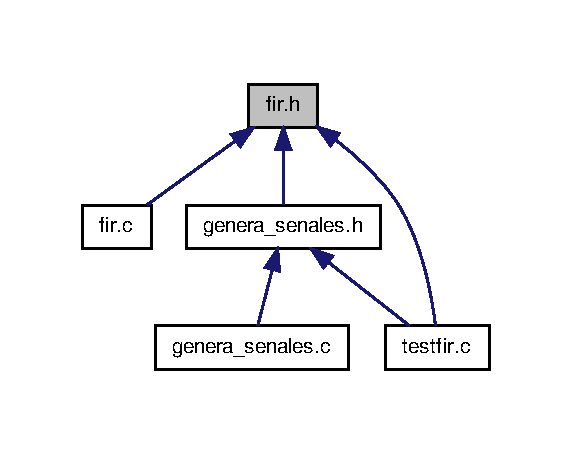
\includegraphics[width=275pt]{fir_8h__dep__incl}
\end{center}
\end{figure}
\subsection*{'defines'}
\begin{DoxyCompactItemize}
\item 
\hypertarget{fir_8h_a54bcb275fff58085463f7abd54bf6459}{
\#define \hyperlink{fir_8h_a54bcb275fff58085463f7abd54bf6459}{TAP\_\-LENGTH}~5}
\label{fir_8h_a54bcb275fff58085463f7abd54bf6459}

\begin{DoxyCompactList}\small\item\em Orden del filtro. \end{DoxyCompactList}\item 
\hypertarget{fir_8h_ac52f13939afa0489aa4ee20f3ace3515}{
\#define \hyperlink{fir_8h_ac52f13939afa0489aa4ee20f3ace3515}{SIGNAL\_\-LENGTH}~15}
\label{fir_8h_ac52f13939afa0489aa4ee20f3ace3515}

\begin{DoxyCompactList}\small\item\em Cantidad de muestras. \end{DoxyCompactList}\end{DoxyCompactItemize}
\subsection*{'typedefs'}
\begin{DoxyCompactItemize}
\item 
\hypertarget{fir_8h_aa0798f7ea0975b143a1d9deac8c05d43}{
typedef float \hyperlink{fir_8h_aa0798f7ea0975b143a1d9deac8c05d43}{sample\_\-t}}
\label{fir_8h_aa0798f7ea0975b143a1d9deac8c05d43}

\begin{DoxyCompactList}\small\item\em Tipo definido para manejar muestras de la señal. \end{DoxyCompactList}\end{DoxyCompactItemize}
\subsection*{Funciones}
\begin{DoxyCompactItemize}
\item 
void \hyperlink{fir_8h_ada2d9b4969eff61ebfbee6ee1bc25206}{ini\_\-fir} (\hyperlink{fir_8h_aa0798f7ea0975b143a1d9deac8c05d43}{sample\_\-t} coefs\mbox{[}$\,$\mbox{]})
\begin{DoxyCompactList}\small\item\em Inicializa el filtro. \end{DoxyCompactList}\item 
\hyperlink{fir_8h_aa0798f7ea0975b143a1d9deac8c05d43}{sample\_\-t} \hyperlink{fir_8h_a2e0d7a8a9b3434fcf994e973dba8349f}{fir} (\hyperlink{fir_8h_aa0798f7ea0975b143a1d9deac8c05d43}{sample\_\-t} $\ast$muestra)
\begin{DoxyCompactList}\small\item\em Aplica filtrado FIR a la muestra de entrada. \end{DoxyCompactList}\end{DoxyCompactItemize}


\subsection{Descripción detallada}
Implementa las funciones de inicialzación del filtro y la función de filtrado. 

\subsection{Documentación de las funciones}
\hypertarget{fir_8h_a2e0d7a8a9b3434fcf994e973dba8349f}{
\index{fir.h@{fir.h}!fir@{fir}}
\index{fir@{fir}!fir.h@{fir.h}}
\subsubsection[{fir}]{\setlength{\rightskip}{0pt plus 5cm}{\bf sample\_\-t} fir (
\begin{DoxyParamCaption}
\item[{{\bf sample\_\-t} $\ast$}]{muestra}
\end{DoxyParamCaption}
)}}
\label{fir_8h_a2e0d7a8a9b3434fcf994e973dba8349f}


Aplica filtrado FIR a la muestra de entrada. 


\begin{DoxyParams}{Parámetros}
{\em muestra} & Puntero a la muestra de la señal de entrada (tipo sample\_\-t) \\
\hline
\end{DoxyParams}
\begin{DoxyReturn}{Devuelve}
Devuelve la muestra de la señal de salida del filtro. 
\end{DoxyReturn}
\hypertarget{fir_8h_ada2d9b4969eff61ebfbee6ee1bc25206}{
\index{fir.h@{fir.h}!ini\_\-fir@{ini\_\-fir}}
\index{ini\_\-fir@{ini\_\-fir}!fir.h@{fir.h}}
\subsubsection[{ini\_\-fir}]{\setlength{\rightskip}{0pt plus 5cm}void ini\_\-fir (
\begin{DoxyParamCaption}
\item[{{\bf sample\_\-t}}]{coefs\mbox{[}$\,$\mbox{]}}
\end{DoxyParamCaption}
)}}
\label{fir_8h_ada2d9b4969eff61ebfbee6ee1bc25206}


Inicializa el filtro. 


\begin{DoxyParams}{Parámetros}
{\em coefs\mbox{[}$\,$\mbox{]}} & Coeficientes del filtro (array de elementos tipos sample\_\-t) \\
\hline
\end{DoxyParams}
\begin{DoxyReturn}{Devuelve}
No tiene salida. 
\end{DoxyReturn}

\hypertarget{genera__senales_8c}{
\section{Referencia del Archivo genera\_\-senales.c}
\label{genera__senales_8c}\index{genera\_\-senales.c@{genera\_\-senales.c}}
}


Genera señales sintéticas para la prueba de la implementación del filtro FIR. Genera señales tipo escalón e impulso.  


{\ttfamily \#include \char`\"{}genera\_\-senales.h\char`\"{}}\par
{\ttfamily \#include $<$stdio.h$>$}\par
Dependencia gráfica adjunta para genera\_\-senales.c:\nopagebreak
\begin{figure}[H]
\begin{center}
\leavevmode
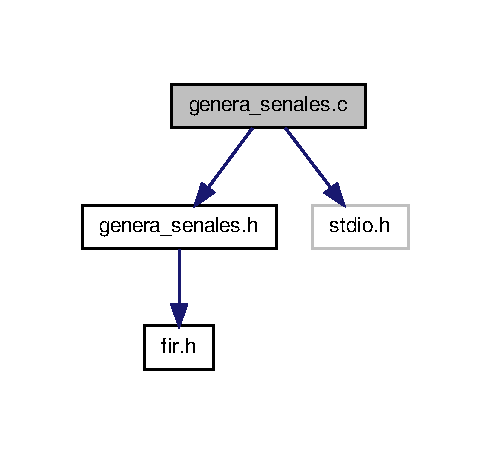
\includegraphics[width=236pt]{genera__senales_8c__incl}
\end{center}
\end{figure}
\subsection*{Funciones}
\begin{DoxyCompactItemize}
\item 
void \hyperlink{genera__senales_8c_ac1831abad5ea41543128b85234b25905}{step} (\hyperlink{fir_8h_aa0798f7ea0975b143a1d9deac8c05d43}{sample\_\-t} $\ast$pu, int tsubida, \hyperlink{fir_8h_aa0798f7ea0975b143a1d9deac8c05d43}{sample\_\-t} altura)
\begin{DoxyCompactList}\small\item\em Genera señales tipo escalón. \end{DoxyCompactList}\item 
void \hyperlink{genera__senales_8c_a2d40e3330ee102e766fe713e8a0262cf}{impulso} (\hyperlink{fir_8h_aa0798f7ea0975b143a1d9deac8c05d43}{sample\_\-t} $\ast$pu, int tsubida, \hyperlink{fir_8h_aa0798f7ea0975b143a1d9deac8c05d43}{sample\_\-t} altura)
\begin{DoxyCompactList}\small\item\em Genera señales tipo impulso. \end{DoxyCompactList}\end{DoxyCompactItemize}


\subsection{Descripción detallada}
Genera señales sintéticas para la prueba de la implementación del filtro FIR. Genera señales tipo escalón e impulso. 

\subsection{Documentación de las funciones}
\hypertarget{genera__senales_8c_a2d40e3330ee102e766fe713e8a0262cf}{
\index{genera\_\-senales.c@{genera\_\-senales.c}!impulso@{impulso}}
\index{impulso@{impulso}!genera_senales.c@{genera\_\-senales.c}}
\subsubsection[{impulso}]{\setlength{\rightskip}{0pt plus 5cm}impulso (
\begin{DoxyParamCaption}
\item[{{\bf sample\_\-t} $\ast$}]{pu, }
\item[{int}]{tsubida, }
\item[{{\bf sample\_\-t}}]{altura}
\end{DoxyParamCaption}
)}}
\label{genera__senales_8c_a2d40e3330ee102e766fe713e8a0262cf}


Genera señales tipo impulso. 


\begin{DoxyParams}{Parámetros}
{\em pu} & Puntero al array de la señal de entrada. \\
\hline
{\em tsubida} & Retardo (en muestras) del impulso. \\
\hline
{\em altura} & Altuda del impulso a generar. \\
\hline
\end{DoxyParams}
\begin{DoxyReturn}{Devuelve}
No tiene salida. 
\end{DoxyReturn}
\hypertarget{genera__senales_8c_ac1831abad5ea41543128b85234b25905}{
\index{genera\_\-senales.c@{genera\_\-senales.c}!step@{step}}
\index{step@{step}!genera_senales.c@{genera\_\-senales.c}}
\subsubsection[{step}]{\setlength{\rightskip}{0pt plus 5cm}step (
\begin{DoxyParamCaption}
\item[{{\bf sample\_\-t} $\ast$}]{pu, }
\item[{int}]{tsubida, }
\item[{{\bf sample\_\-t}}]{altura}
\end{DoxyParamCaption}
)}}
\label{genera__senales_8c_ac1831abad5ea41543128b85234b25905}


Genera señales tipo escalón. 


\begin{DoxyParams}{Parámetros}
{\em pu} & Puntero al array de la señal de entrada. \\
\hline
{\em tsubida} & Retardo (en muestras) del escalón. \\
\hline
{\em altura} & Altura del escalón a generar. \\
\hline
\end{DoxyParams}
\begin{DoxyReturn}{Devuelve}
No tiene salida. 
\end{DoxyReturn}

\hypertarget{genera__senales_8h}{
\section{Referencia del Archivo genera\_\-senales.h}
\label{genera__senales_8h}\index{genera\_\-senales.h@{genera\_\-senales.h}}
}


Genera señales sintéticas para la prueba de la implementación del filtro FIR. Genera señales tipo escalón e impulso.  


{\ttfamily \#include \char`\"{}fir.h\char`\"{}}\par
Dependencia gráfica adjunta para genera\_\-senales.h:\nopagebreak
\begin{figure}[H]
\begin{center}
\leavevmode
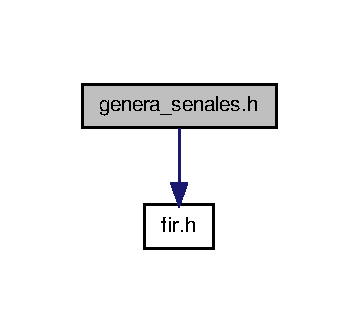
\includegraphics[width=172pt]{genera__senales_8h__incl}
\end{center}
\end{figure}
Gráfico de los archivos que directa o indirectamente incluyen a este archivo:
\nopagebreak
\begin{figure}[H]
\begin{center}
\leavevmode
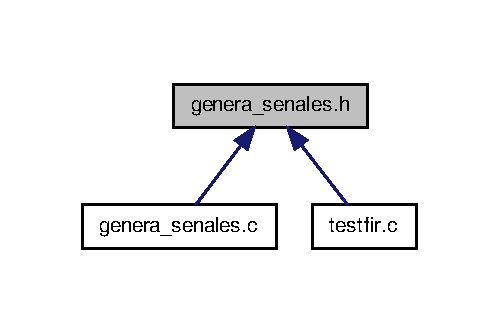
\includegraphics[width=240pt]{genera__senales_8h__dep__incl}
\end{center}
\end{figure}
\subsection*{Funciones}
\begin{DoxyCompactItemize}
\item 
void \hyperlink{genera__senales_8h_a10df71dbee03eb4676d58cbd1fa25042}{step} (\hyperlink{fir_8h_aa0798f7ea0975b143a1d9deac8c05d43}{sample\_\-t} $\ast$pu, int tsubida, \hyperlink{fir_8h_aa0798f7ea0975b143a1d9deac8c05d43}{sample\_\-t} altura)
\begin{DoxyCompactList}\small\item\em Genera señales tipo escalón. \end{DoxyCompactList}\item 
void \hyperlink{genera__senales_8h_a40c9b355ff90e9490a42d6cea8d0e440}{impulso} (\hyperlink{fir_8h_aa0798f7ea0975b143a1d9deac8c05d43}{sample\_\-t} $\ast$pu, int tsubida, \hyperlink{fir_8h_aa0798f7ea0975b143a1d9deac8c05d43}{sample\_\-t} altura)
\begin{DoxyCompactList}\small\item\em Genera señales tipo impulso. \end{DoxyCompactList}\end{DoxyCompactItemize}


\subsection{Descripción detallada}
Genera señales sintéticas para la prueba de la implementación del filtro FIR. Genera señales tipo escalón e impulso. 

\subsection{Documentación de las funciones}
\hypertarget{genera__senales_8h_a40c9b355ff90e9490a42d6cea8d0e440}{
\index{genera\_\-senales.h@{genera\_\-senales.h}!impulso@{impulso}}
\index{impulso@{impulso}!genera_senales.h@{genera\_\-senales.h}}
\subsubsection[{impulso}]{\setlength{\rightskip}{0pt plus 5cm}void impulso (
\begin{DoxyParamCaption}
\item[{{\bf sample\_\-t} $\ast$}]{pu, }
\item[{int}]{tsubida, }
\item[{{\bf sample\_\-t}}]{altura}
\end{DoxyParamCaption}
)}}
\label{genera__senales_8h_a40c9b355ff90e9490a42d6cea8d0e440}


Genera señales tipo impulso. 


\begin{DoxyParams}{Parámetros}
{\em pu} & Puntero al array de la señal de entrada. \\
\hline
{\em tsubida} & Retardo (en muestras) del impulso. \\
\hline
{\em altura} & Altuda del impulso a generar. \\
\hline
\end{DoxyParams}
\begin{DoxyReturn}{Devuelve}
No tiene salida. 
\end{DoxyReturn}
\hypertarget{genera__senales_8h_a10df71dbee03eb4676d58cbd1fa25042}{
\index{genera\_\-senales.h@{genera\_\-senales.h}!step@{step}}
\index{step@{step}!genera_senales.h@{genera\_\-senales.h}}
\subsubsection[{step}]{\setlength{\rightskip}{0pt plus 5cm}void step (
\begin{DoxyParamCaption}
\item[{{\bf sample\_\-t} $\ast$}]{pu, }
\item[{int}]{tsubida, }
\item[{{\bf sample\_\-t}}]{altura}
\end{DoxyParamCaption}
)}}
\label{genera__senales_8h_a10df71dbee03eb4676d58cbd1fa25042}


Genera señales tipo escalón. 


\begin{DoxyParams}{Parámetros}
{\em pu} & Puntero al array de la señal de entrada. \\
\hline
{\em tsubida} & Retardo (en muestras) del escalón. \\
\hline
{\em altura} & Altura del escalón a generar. \\
\hline
\end{DoxyParams}
\begin{DoxyReturn}{Devuelve}
No tiene salida. 
\end{DoxyReturn}

\hypertarget{testfir_8c}{
\section{Referencia del Archivo testfir.c}
\label{testfir_8c}\index{testfir.c@{testfir.c}}
}


Programa para probar el filtro FIR implementado.  


{\ttfamily \#include \char`\"{}fir.h\char`\"{}}\par
{\ttfamily \#include \char`\"{}genera\_\-senales.h\char`\"{}}\par
{\ttfamily \#include $<$stdio.h$>$}\par
Dependencia gráfica adjunta para testfir.c:
\nopagebreak
\begin{figure}[H]
\begin{center}
\leavevmode
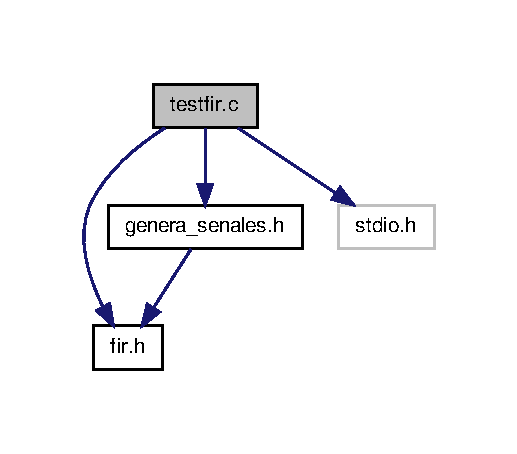
\includegraphics[width=248pt]{testfir_8c__incl}
\end{center}
\end{figure}
\subsection*{Funciones}
\begin{DoxyCompactItemize}
\item 
int \hyperlink{testfir_8c_a51af30a60f9f02777c6396b8247e356f}{main} ()
\begin{DoxyCompactList}\small\item\em Prueba de los módulos implementados. \end{DoxyCompactList}\end{DoxyCompactItemize}


\subsection{Descripción detallada}
Programa para probar el filtro FIR implementado. 

\subsection{Documentación de las funciones}
\hypertarget{testfir_8c_a51af30a60f9f02777c6396b8247e356f}{
\index{testfir.c@{testfir.c}!main@{main}}
\index{main@{main}!testfir.c@{testfir.c}}
\subsubsection[{main}]{\setlength{\rightskip}{0pt plus 5cm}main (
\begin{DoxyParamCaption}
{}
\end{DoxyParamCaption}
)}}
\label{testfir_8c_a51af30a60f9f02777c6396b8247e356f}


Prueba de los módulos implementados. 

\begin{DoxyReturn}{Devuelve}
No tiene salida. 
\end{DoxyReturn}


Señal de entrada.

Señal de salida.

Coeficientes del FIR.

Retardo de la señal de entrada (en muestras).

Altura de la señal de entrada 



Gráfico de llamadas para esta función:
\nopagebreak
\begin{figure}[H]
\begin{center}
\leavevmode
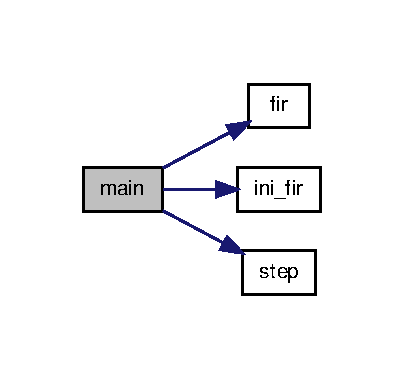
\includegraphics[width=194pt]{testfir_8c_a51af30a60f9f02777c6396b8247e356f_cgraph}
\end{center}
\end{figure}



\printindex
\end{document}
